\begin{figure}[th]
\begin{center}
\begin{scriptsize}
\begin{sc}
\begin{tikzpicture}[node distance=2ex, auto]
\tikzstyle{every node}=[font=\footnotesize]

\newlength{\stepimage}
\setlength{\stepimage}{6em}

\tikzstyle{module} = [rectangle, rounded corners, minimum width=2.5cm, minimum height=0.5cm,text centered, draw=black, fill=blue!20]
\tikzstyle{largemodule} = [rectangle, rounded corners, minimum width=3.5cm, minimum height=1cm,text centered, draw=black, fill=blue!20]
\tikzstyle{inputoutput} = [rectangle, rounded corners,text centered, draw=black,inner sep=5px]
\tikzstyle{arrow} = [ultra thick,->,>=stealth]
\tikzstyle{pict} = [inner sep=0px]

\node [module] (task) {\makecell[c]{Task:\\locate a predator}};

\node [inputoutput, left=of task] (human)  {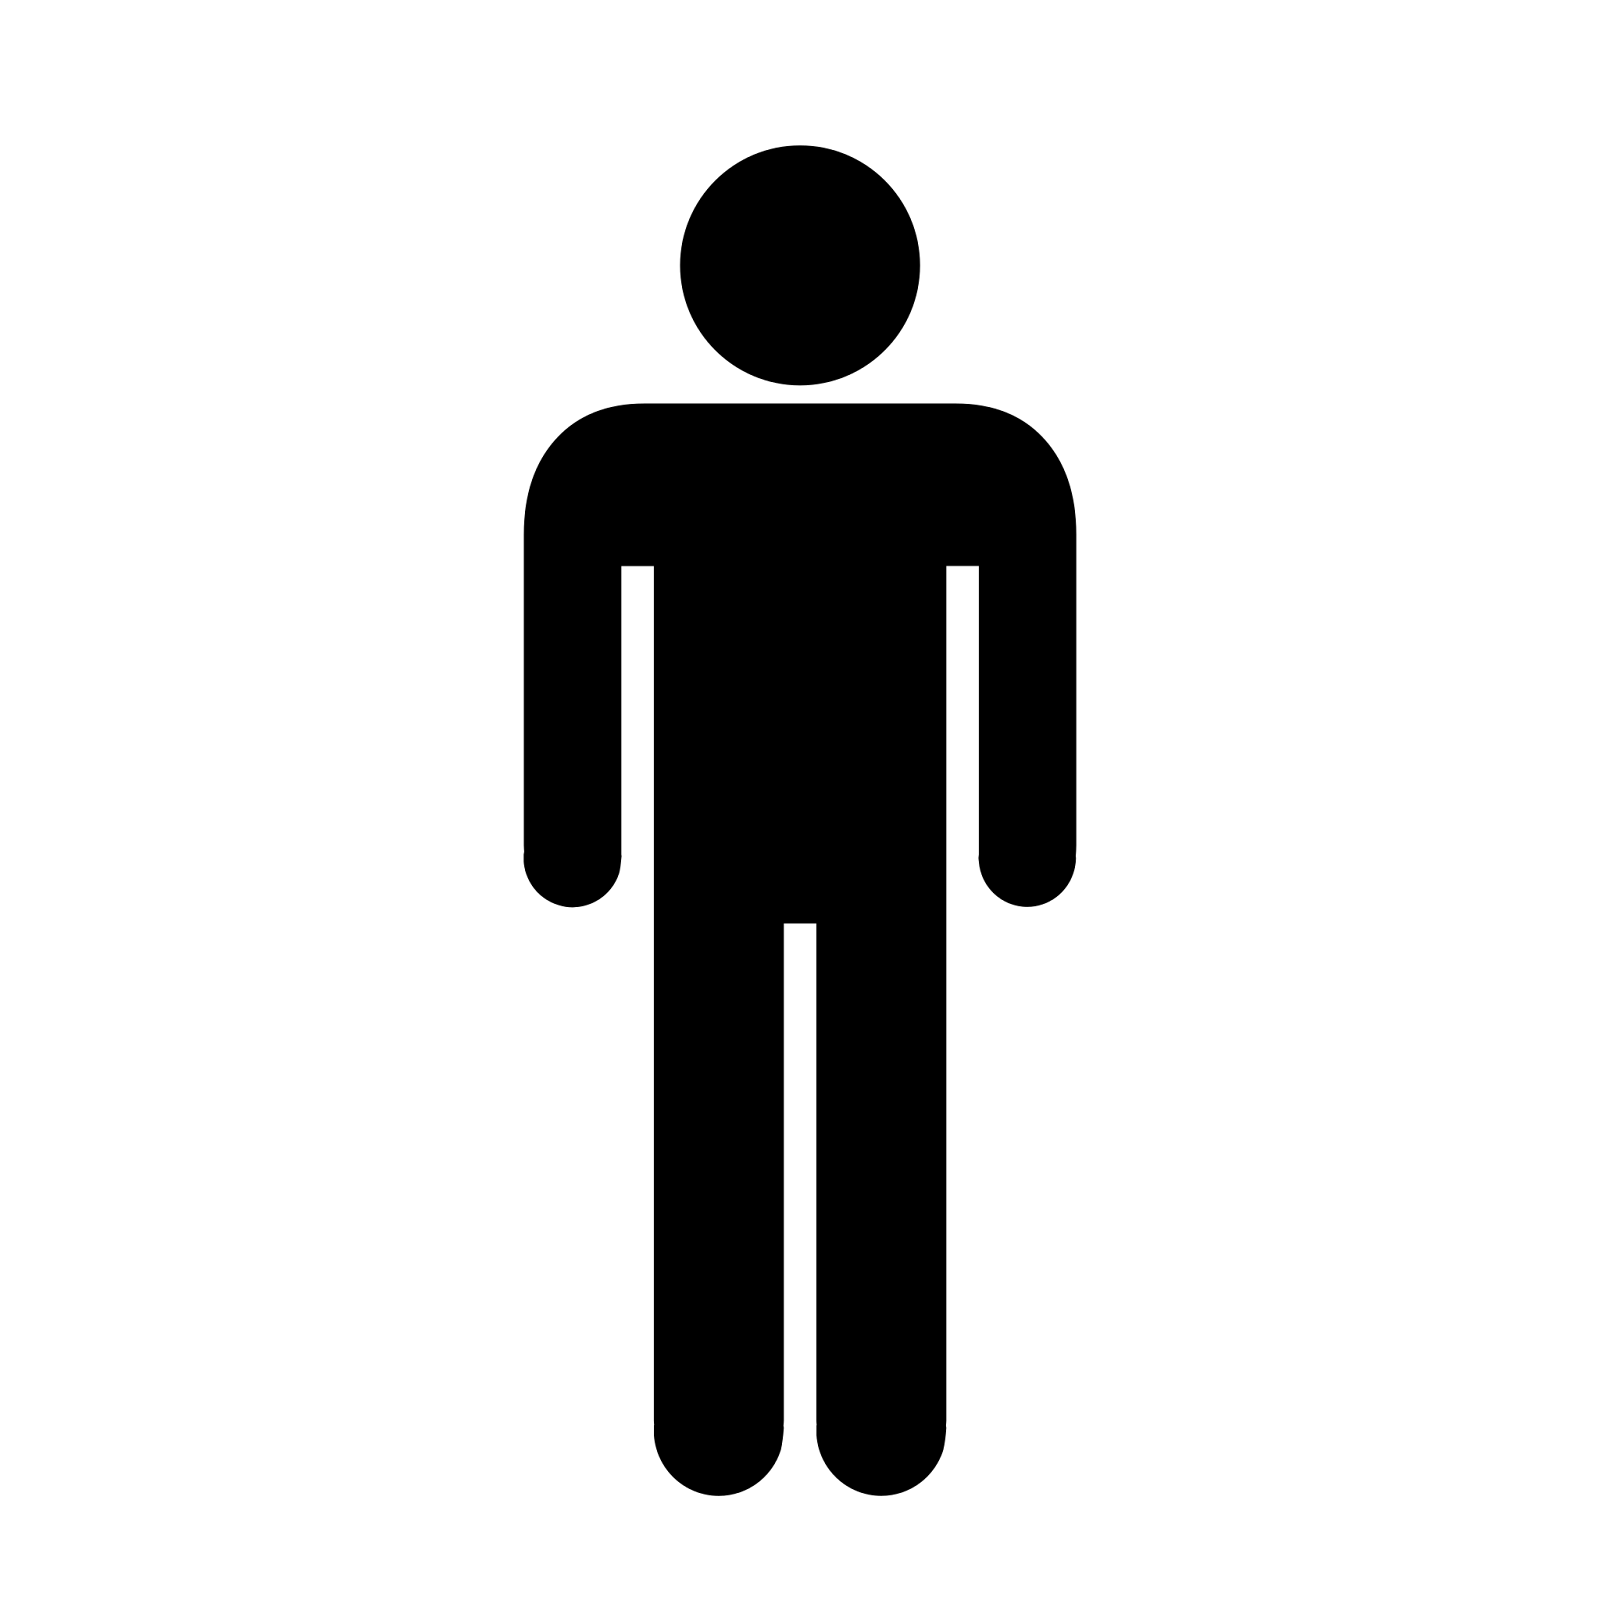
\includegraphics[height=3em]{fig_poster/overview/images/human.png}};
\node [inputoutput, right=of task] (robot)  {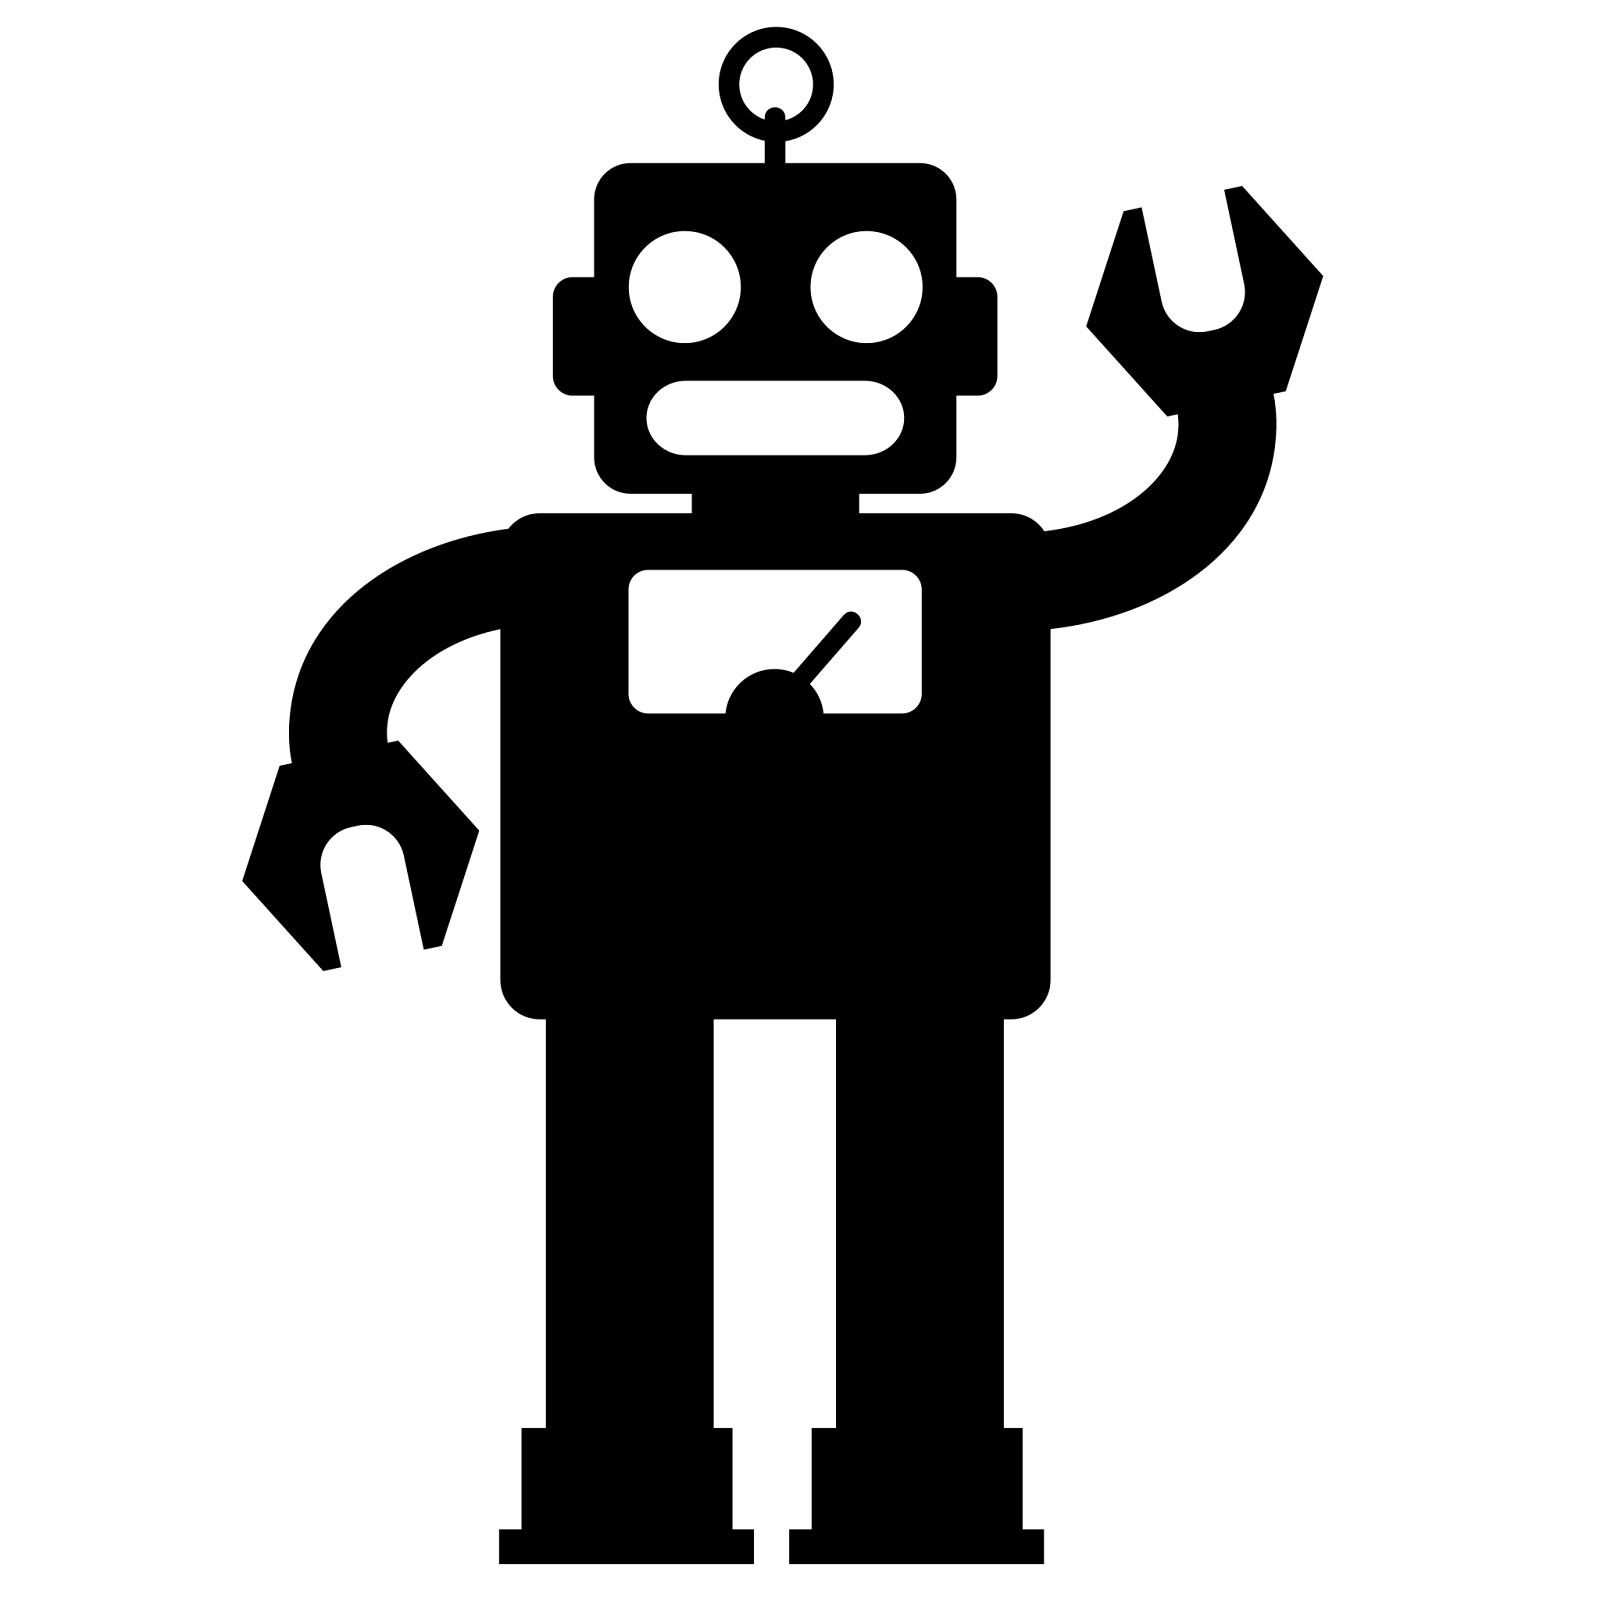
\includegraphics[height=3em]{fig_poster/overview/images/robot.png}};

\node [pict, below=of human, label={[align=right]left:An animal\\on the left}] (h1)  {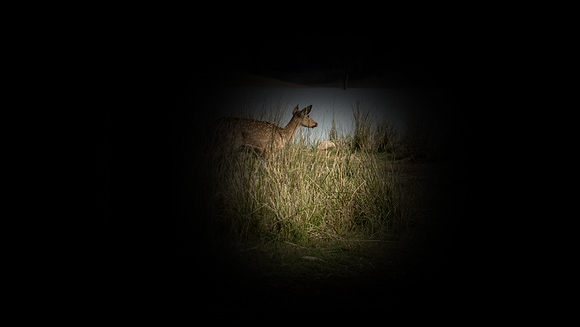
\includegraphics[width=\stepimage]{fig_poster/overview/images/h1.jpg}};
\node [pict, below=of h1, label={[align=right]left:Antelope is running\\to the right}] (h2)  {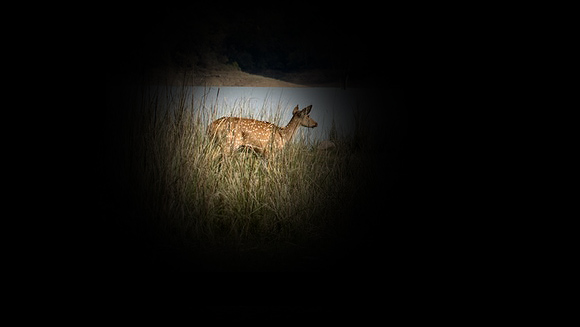
\includegraphics[width=\stepimage]{fig_poster/overview/images/h2.jpg}};
\node [pict, below=of h2, label={[align=right]left:Something orange \\is down-left}] (h3)  {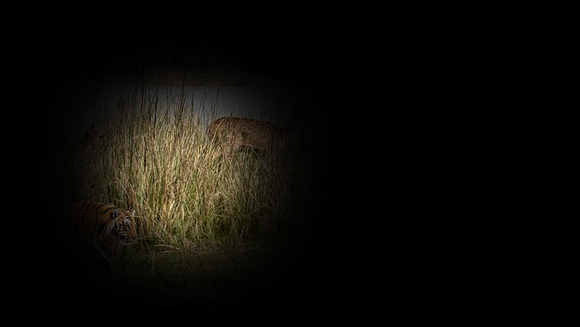
\includegraphics[width=\stepimage]{fig_poster/overview/images/h3.jpg}};
\node [pict, below=of h3, label={[align=right]left:Found a tiger!}] (h4)  {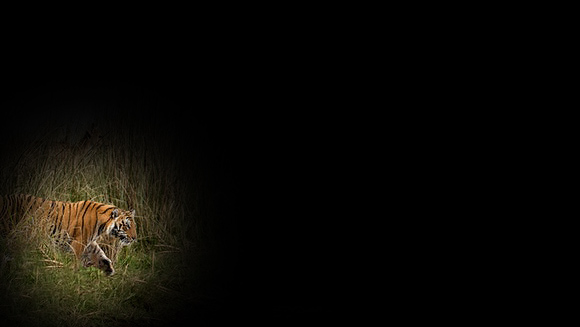
\includegraphics[width=\stepimage]{fig_poster/overview/images/h4.jpg}};

\node [pict, below=of robot, label={[align=left]right:No animal}] (r1)  {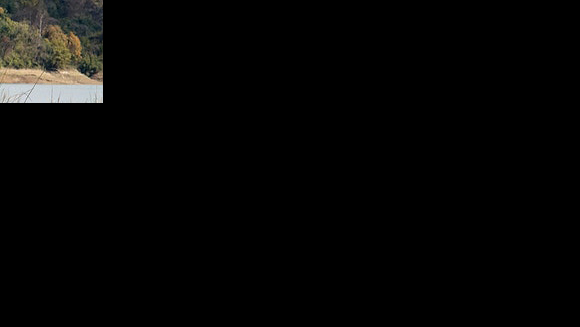
\includegraphics[width=\stepimage]{fig_poster/overview/images/r1.jpg}};
\node [pict, below=of r1, label={[align=left]right:No animal}] (r2)  {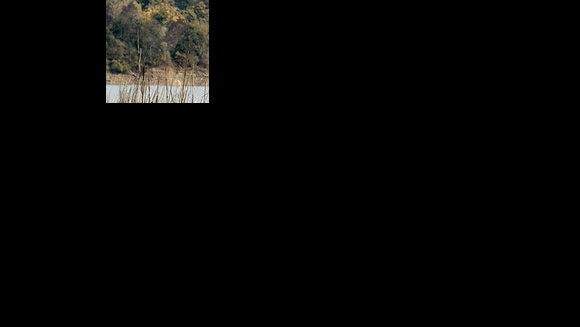
\includegraphics[width=\stepimage]{fig_poster/overview/images/r2.jpg}};
\node [pict, below=of r2, label={[align=left]right:No animal}] (r3)  {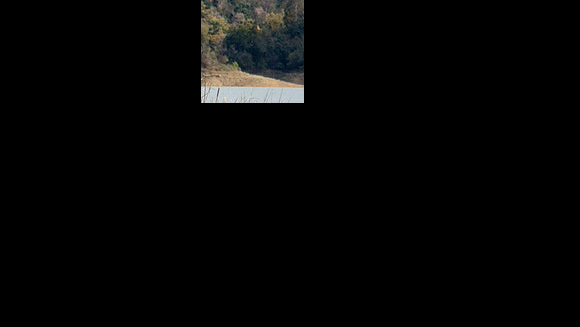
\includegraphics[width=\stepimage]{fig_poster/overview/images/r3.jpg}};
\node [inputoutput, below=of r3, label={[align=left]right:Several step later}] (r4)  {$\dotsc$};
\node [pict, below=of r4, label={[align=center]right:Not a predator}] (r5)  {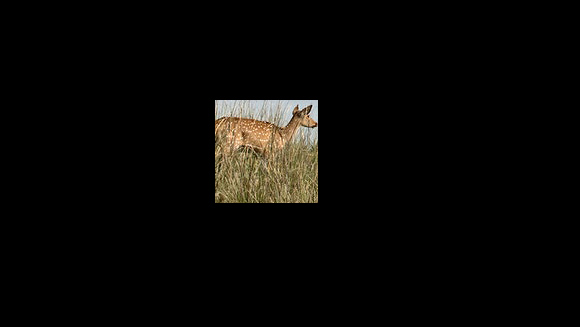
\includegraphics[width=\stepimage]{fig_poster/overview/images/r4.jpg}};
\node [inputoutput, below=of r5, label={[align=left]right:Several step later}] (r6)  {$\dotsc$};
\node [pict, below=of r6, label={[align=left]right:Found a tiger!}] (r7)  {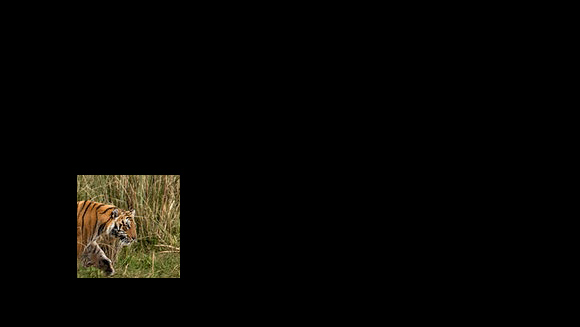
\includegraphics[width=\stepimage]{fig_poster/overview/images/r5.jpg}};

\draw [arrow] (task) -- (human);
\draw [arrow] (task) -- (robot);

\draw [arrow] (human) -- (h1);
\draw [arrow] (h1) -- (h2) node[midway, right] {Look left};
\draw [arrow] (h2) -- (h3) node[midway, right] {Look left};
\draw [arrow] (h3) -- (h4) node[midway, right] {Look down-left};

\draw [arrow] (robot) -- (r1);
\draw [arrow] (r1) -- (r2) node[midway, left] {Look next};
\draw [arrow] (r2) -- (r3) node[midway, left] {Look next};
\draw [arrow] (r3) -- (r4) node[midway, left] {Look next};
\draw [arrow] (r4) -- (r5) node[midway, left] {Look next};
\draw [arrow] (r5) -- (r6) node[midway, left] {Look next};
\draw [arrow] (r6) -- (r7) node[midway, left] {Look next};


\end{tikzpicture}
\end{sc}
\end{scriptsize}
\end{center}
    \caption{\textbf{Visual exploration -- human versus AI}: Humans naturally visually explore surrounding environment, using already observed areas as clues to where the wanted object can be located~\cite{hayhoe2005eye}. At the same time, common state-of-the-art artificial intelligence solutions analyze all available data, which is inefficient and waste time and computational resources. In this project, we introduce a novel Active Visual Exploration method, enabling AI agents to efficiently explore their environment.}
    \label{fig:overview}
\end{figure}
